\documentclass[12pt,a4paper,twoside,fleqn]{article}
\usepackage[inner=29mm,outer=26mm,top=28mm,bottom=29mm,headheight=16pt]{geometry}
\usepackage[T1]{fontenc}
\usepackage{newtxtext}
\usepackage{amsmath,amsthm,mathtools,newtxmath,microtype}
\usepackage{booktabs,tabularx,array,graphicx,float,enumitem,titlesec,fancyhdr,placeins}
\usepackage[round,authoryear]{natbib}
\renewcommand{\bibfont}{\small\raggedright}
\usepackage[hidelinks]{hyperref}
\hypersetup{bookmarksdepth=2,pdftitle={Coexistence, stability and bifurcation},pdfsubject={Project 3H (Version B)}}
\urlstyle{same}
\newcommand{\doi}[1]{\href{https://doi.org/#1}{\textnormal{#1}}}
\newcommand{\DOIprefix}{doi:\,}
\pagestyle{fancy}\fancyhf{}
\fancyhead[LE,RO]{\small\thepage}
\fancyhead[LO]{\small Weak-Allee growth and a foraging-arena response}
\fancyhead[RE]{\small Coexistence, stability and bifurcation}
\fancypagestyle{plain}{\fancyhf{}\fancyfoot[C]{\thepage}\renewcommand{\headrulewidth}{0pt}}
\titleformat{\section}{\large\bfseries}{\thesection.}{.65em}{}
\titleformat{\subsection}{\normalsize\itshape}{\thesubsection.}{.65em}{}
\setlength{\mathindent}{1.7em}
\setlength{\emergencystretch}{1.5em}
\setlength{\intextsep}{12pt}
\setlist[enumerate,1]{label=\textup{(\roman*)},leftmargin=2.2em,topsep=4pt,itemsep=3pt}
\setcounter{tocdepth}{1}
\newcolumntype{Y}{>{\raggedright\arraybackslash}X}
\newtheoremstyle{journal}{9pt}{7pt}{\itshape}{}{\bfseries}{.}{.45em}{\thmname{#1}\thmnumber{ #2}\thmnote{ \textup{(#3)}}}
\theoremstyle{journal}
\newtheorem{theorem}{Theorem}
\newtheorem{lemma}{Lemma}
\newtheorem{proposition}{Proposition}
\newtheorem{corollary}{Corollary}
\newcommand{\claim}[1]{{\normalfont\bfseries\boldmath #1}}
\renewcommand{\proofname}{\normalfont\bfseries Proof}
\newcommand{\dd}{\mathrm{d}}
\newcommand{\tr}{\operatorname{tr}}
\newcommand{\Real}{\operatorname{Re}}
\newcommand{\Q}{\mathcal Q}
\newcommand{\Det}{\mathcal D}
\newcommand{\pos}{\mathbb R_{>0}^{\,2}}
\raggedbottom

\begin{document}
\thispagestyle{plain}
{\raggedright\noindent\LARGE\bfseries Coexistence, stability and bifurcation in a predator--prey model with weak Allee growth and a foraging-arena response\par}
\vspace{.8em}{\noindent\large Project 3H (Version B)\par}\vspace{1.05em}
\noindent\textbf{Executive summary.}
The invasion ratio \(R=emk/(d\beta)\) separates predator extinction from uniform persistence. When \(R>1\), an explicit cubic classifies the positive equilibria. Depending on its roots and the local stability conditions, the model can have a single attracting coexistence state, two stable states with different basins, or a periodic attractor. We establish sufficient global conditions using Lyapunov functions, a Dulac test and a Li\'enard transformation. We identify transcritical, saddle-node, cusp, Hopf, Bogdanov--Takens and generalized Hopf bifurcations. Numerical examples show how the trajectories change across thresholds in predation and carrying capacity and how the two basins are separated. Three literature-informed scenarios compare prey growth rates within a common parameter setting. Local stochastic examples give mean-square stability conditions for independent white noise and common colored noise.

\medskip\noindent\textbf{Keywords}\quad Weak Allee effect \(\cdot\) Predator interference \(\cdot\) Phase portraits \(\cdot\) Bifurcation
\tableofcontents
\clearpage

\section{Introduction}
A weak Allee effect allows prey per-capita growth to increase at low density while remaining positive at zero density. Predator interference acts through a foraging-arena response in which intake per predator decreases as predator density rises. Together these mechanisms change both the conditions for predator invasion and the possible outcomes after invasion. In particular, persistence can be consistent with more than one coexistence state or with sustained oscillation.

\citet{haque11} organized the analysis of a predator--prey system around permanence, local and global stability, bifurcation, stochastic stability, and numerical examples. We follow that programme for the ordinary differential equation displayed in the Version B brief \citep{brief}. Haque's Beddington--DeAngelis response depends on both prey and predator density in its denominator, and his main numerical model includes predator self-limitation. Here the denominator is \(\beta+y\) and the displayed predator equation contains linear mortality. These differences change the coexistence equation and the bifurcation thresholds. \citet{haque09} gives a complementary comparison for an explicitly ratio-dependent response.

The analytical sections identify the hypotheses for each qualitative result. The numerical sections pair parameter values and phase portraits with equilibrium, stability or return-map checks. We use constructed cases to isolate dynamical mechanisms and literature-informed cases to examine sensitivity to prey growth. Appendix~\ref{sec:figurecode} gives the path of the Python script for each figure.

\section{Model formulation and fundamental properties}\label{sec:model}
Let \(x(t),y(t)\) denote the prey and predator densities. We study the system displayed as equation (1.1) in the Version B brief \citep{brief}, with strictly positive initial densities:
\begin{equation}\label{eq:ode}
 \begin{aligned}
 \frac{\dd x}{\dd t}&=xF(x)-\frac{mxy}{\beta+y}=f(x,y),\\
 \frac{\dd y}{\dd t}&=\frac{emxy}{\beta+y}-dy=g(x,y),\\
 F(x)&=r(1-x/k)(1+\alpha x).
 \end{aligned}
\end{equation}
The printed equations correspond to a zero coefficient on the separate predator self-competition term mentioned in the brief's prose. Interference still enters through \(y\) in the denominator of the intake rate. Prey grow at the positive per-capita rate \(r\) at zero density. This rate initially rises with density when \(\alpha k>1\). It decreases for \(x>0\) when \(\alpha k\le 1\).

\begin{table}[tbp]\centering
\caption{Positive dimensional parameters and their role in the scaling.}\label{tab:param}
\begin{tabularx}{\linewidth}{@{}lYl@{}}\toprule
Parameter & Meaning & Scaled quantity \\ \midrule
\(r\) & Intrinsic prey growth rate & \(\tau=rt\) \\
\(k\) & Prey carrying capacity & \(X=x/k\) \\
\(\alpha\) & Low-density facilitation coefficient for prey & \(A=\alpha k\) \\
\(m\) & Predation rate coefficient & \(M=m/r\) \\
\(\beta\) & Predator density at half-saturation of total intake per prey & \(Y=y/\beta\) \\
\(e\) & Predator density gained per unit of prey density consumed & \(R=emk/(d\beta)\) \\
\(d\) & Predator mortality rate & \(D=d/r\) \\
\bottomrule\end{tabularx}
\end{table}

With \(p(X)=(1-X)(1+AX)\), the scaled model is
\begin{equation}\label{eq:scaled}
 X'=X\left[p(X)-\frac{MY}{1+Y}\right],\qquad
 Y'=DY\left[\frac{RX}{1+Y}-1\right],
\end{equation}
where \( '\) denotes differentiation with respect to \(\tau\) on state variables. Given \(r,k,\beta\) and positive \(A,M,R,D\), the inverse map is
\(\alpha=A/k,\ m=rM,\ d=rD,\ e=DR\beta/(Mk)\).
The ratio \(R\) compares the predator's birth and death rates when it is rare and prey are at carrying capacity.

\begin{theorem}[Positivity, continuation, and bounds]\label{thm:bounds}
The nonnegative quadrant is forward invariant, and positive solutions remain positive for all \(t\ge0\). Set \(W=ex+y\) and \(B_0=\max_{x\ge0} ex[F(x)+d]\). Then
\[
 W(t)\le W(0)e^{-dt}+(B_0/d)(1-e^{-dt}),\qquad
 x(t)\le\max\{x(0),k\}.
\]
Moreover, \(\limsup_{t\to\infty}x(t)\le k\) and
\(\limsup_{t\to\infty}y(t)\le\beta\max\{0,R-1\}\).
\end{theorem}
\begin{proof}
Both axes are invariant by uniqueness. The leading cubic coefficient in \(ex[F(x)+d]\) is negative, and \(\dot W=-dW+ex[F(x)+d]\). Its upper bound gives continuation on the smooth domain \(y>-\beta\). Compare the prey equation with \(\dot x=xF(x)\). Once \(x\le k+\varepsilon\), compare the predator equation with \(\dot z=z[em(k+\varepsilon)/(\beta+z)-d]\), and then let \(\varepsilon\downarrow0\).
\end{proof}

\begin{theorem}[Exact persistence threshold]\label{thm:per}
For positive initial densities and \(R\le1\), \((x(t),y(t))\to(k,0)\). For \(R>1\), both species are uniformly persistent. There is a parameter-dependent \(\delta_*>0\) such that \(\liminf_{t\to\infty}\min\{x(t),y(t)\}\ge\delta_*\).
\end{theorem}
\begin{proof}
For \(R\le1\) the predator bound gives \(y\to0\). Below any \(b<k\), the prey per-capita growth eventually exceeds \(\tfrac12\min_{[0,b]}F>0\). This gives \(\liminf x\ge k\).

For \(R>1\), put \(\xi=k/R,\ b_0=\xi/2,\ \gamma=d/2\). Eventually \(y\le\beta(2R-1)\). On an excursion with \(x<b_0\), the predator decays at rate at least \(\gamma\), and integrating the prey per-capita loss gives an eventual prey floor \(\delta_x=b_0(2R)^{-m/\gamma}\); see \eqref{eq:floorentropy}. If the solution starts below \(b_0\) when the predator bound takes effect, this decay forces it to reach \(b_0\) in finite time. Choose \(b\in(\xi,k)\) and \(\eta>0\) small enough that prey recover to \(b\) in time at most \(2\log(b/\delta_x)/\min_{[0,b]}F\) while \(y\le\eta\), and that predator growth is positive there once \(x\ge b\). Since its per-capita loss is at most \(d\) during prey recovery, every later excursion below \(\eta\) has a common positive lower bound.
\end{proof}

\section{Equilibria and their classification}\label{sec:eq}

\subsection{Boundary and positive equilibria}
\begin{lemma}[Feasibility]\label{lem:feas}
The boundary equilibria are \(E_0=(0,0)\) and \(E_1=(k,0)\). Any positive equilibrium \(E^*=(x^*,y^*)\) has \(x^*\) a root of \(Q=0\) in \((C/m,k)\) and \(y^*=emx^*/d-\beta\), where
\begin{equation}\label{eq:Q}
 a=\frac{r\alpha}{k},\quad
 L_0=k-\frac{1}{\alpha},\quad
 C=\frac{d\beta}{e},\qquad
 Q(x)=-ax^3+aL_0x^2+(r-m)x+C.
\end{equation}
\end{lemma}
\begin{proof}
The invariant axes give the boundary equilibria. In the interior, \(g=0\) gives \(y=emx/d-\beta\). Substitution into \(f=0\) gives \(F(x)=m-C/x\), or \(Q(x)=x[F(x)-m]+C=0\). Positivity requires \(x>C/m\) and \(x<k\), and every root in this interval solves both equations. For \(R>1\), \(Q(C/m)>0>Q(k)\); \(Q\) is positive on \([0,C/m]\) and negative on \([k,\infty)\). For \(R\le1\) the feasible interval is empty.
\end{proof}

\subsection{Coordinates and multiplicity}
Divide \(-Q\) by \(a\), with \(b_2=-L_0,\ b_1=(m-r)/a,\ b_0=-C/a\). The shift \(x=z-b_2/3\) gives \(z^3+p_c z+q_c=0\), where
\[
 p_c=b_1-b_2^2/3,\quad q_c=2b_2^3/27-b_2b_1/3+b_0,\quad
 \Delta_c=(q_c/2)^2+(p_c/3)^3.
\]
The discriminant is \(-108\Delta_c\). For \(\Delta_c>0\), the real root is
\[
 z=\sqrt[3]{-q_c/2+\sqrt{\Delta_c}}+\sqrt[3]{-q_c/2-\sqrt{\Delta_c}},
\]
where both cube roots are real. For \(\Delta_c<0\), \(p_c<0\) and the three real roots are
\[
 z_j=2\sqrt{-p_c/3}\cos\!\left[
 \tfrac13\arccos\!\left(\frac{-q_c/2}{(-p_c/3)^{3/2}}\right)-\tfrac{2\pi j}{3}
 \right],\qquad j=0,1,2.
\]
For \(\Delta_c=0\), let \(u=\sqrt[3]{-q_c/2}\). The roots are \(2u\) and the double root \(-u\) if \(u\ne0\), and the triple root \(0\) if \(u=0\). Apply Lemma~\ref{lem:feas} to \(x=z-b_2/3\) in each case to find the feasible coordinates.

The feasible branch can also be read from
\[
 m=\mathcal M(x)=F(x)+C/x,\qquad
 x^2\mathcal M'(x)=a x^2(L_0-2x)-C,\qquad 0<x<k.
\]
Its endpoints are \(+\infty\) at zero and \(m_c=C/k\) at \(k\). When \(L_0>0\), the maximum of \(a x^2(L_0-2x)\) occurs at \(x_c=L_0/3\) and equals \(C_{\mathrm{crit}}=aL_0^3/27\). If \(0<C<C_{\mathrm{crit}}\), the two solutions \(x_-<x_+\) to \(a x^2(L_0-2x)=C\) in \((0,L_0/2)\) yield
\[
 m_\pm=\mathcal M(x_\pm)=r+2aL_0x_\pm-3ax_\pm^2.
\]
At \(C=C_{\mathrm{crit}}\), the two turning points merge at \(m_*=r+aL_0^2/3\).

\begin{theorem}[Complete coexistence classification]\label{thm:roots}
Positive equilibria exist exactly when \(R>1\), or equivalently \(m>m_c\). Their number and multiplicities are given in Table~\ref{tab:count}.
At \(m=m_c\), \(x=k\) is a simple root on the axial boundary.
\end{theorem}
The counts follow by intersecting the horizontal line \(m\) with the monotone pieces of \(\mathcal M\). For \(0<C<C_{\mathrm{crit}}\) the successive slope signs are \(-,+,-\). At \(m=m_c\), \(Q'(k)=kF'(k)-C/k<0\).

\begin{table}[tbp]\centering
\caption{Distinct, feasible positive equilibria and their multiplicities in increasing order of prey density.}\label{tab:count}
\begin{tabularx}{\linewidth}{@{}lYcl@{}}\toprule
Shape regime & Predation coefficient & Count & Multiplicities \\ \midrule
Any & \(m\le m_c\) & 0 & --- \\
\(L_0\le0\) or \(C>C_{\mathrm{crit}}\) & \(m>m_c\) & 1 & simple \\
\(L_0>0,\ C=C_{\mathrm{crit}}\) & \(m>m_c,\ m\ne m_*\) & 1 & simple \\
 & \(m=m_*\) & 1 & triple \\
\(L_0>0,\ C<C_{\mathrm{crit}}\) & \(m_c<m<m_-\) or \(m>m_+\) & 1 & simple \\
 & \(m=m_-\) & 2 & double, simple \\
 & \(m_-<m<m_+\) & 3 & simple, simple, simple \\
 & \(m=m_+\) & 2 & simple, double \\
\bottomrule\end{tabularx}
\end{table}

\subsection{Effects of the biological parameters}
At a simple root \(s\), with all other dimensional inputs fixed,
\begin{equation}\label{eq:slopes}
 \begin{aligned}
 s_\mu&=-Q_\mu/Q_x,\\
 (Q_\alpha,Q_\beta,Q_m,Q_k,Q_d)
 &=\left(rs^2(1-s/k),\ d/e,\ -s,\ rs^2(1+\alpha s)/k^2,\ \beta/e\right).
 \end{aligned}
\end{equation}
On a descending branch, prey density increases locally with \(\alpha,\beta,k\) and decreases with \(m\). An ascending root has the reverse sensitivities. Larger \(\beta\) raises the invasion threshold \(m_c\) and brings the two folds together by increasing \(C\) toward \(C_{\mathrm{crit}}\). Increasing \(\alpha\) or \(k\) raises \(C_{\mathrm{crit}}\) when \(A>1\). These simple-root derivatives need not extend to a fold.

\section{Local stability}\label{sec:local}
We classify each equilibrium separately, following the organization of \citet[Section~3.2]{haque11}. The Jacobian of \eqref{eq:ode} is
\begin{equation}\label{eq:jac}
 J(x,y)=\begin{pmatrix}
 F+xF'-my/(\beta+y)&-m\beta x/(\beta+y)^2\\
 emy/(\beta+y)&em\beta x/(\beta+y)^2-d
 \end{pmatrix}.
\end{equation}

\subsection{Extinction equilibrium \texorpdfstring{\(E_0=(0,0)\)}{E0}}
The eigenvalues are \(r\) and \(-d\), so \(E_0\) is always a saddle. Its local unstable and stable manifolds coincide with the prey and predator axes, respectively.

\subsection{Predator-free equilibrium \texorpdfstring{\(E_1=(k,0)\)}{E1}}
The Jacobian is triangular, with diagonal entries \(-\kappa=-r(1+\alpha k)\) and \(d(R-1)\). Thus \(E_1\) is a stable node for \(R<1\) and a saddle for \(R>1\). The former is defective at \(d(1-R)=\kappa\), since the upper off-diagonal entry is nonzero. At \(R=1\), the center dynamics in \(v=y\) are
\(\dot v=-[d(1+m/\kappa)/\beta]v^2+O(v^3)\). Attraction holds on the biological side. Section~\ref{sec:bif} derives this center equation and the exchange of stability.

\subsection{Positive equilibria \texorpdfstring{\(E^*=(x^*,y^*)\)}{E*}}\label{sec:singlelocal}
At the root \(x_i\) put \(F_i=F(x_i)\), \(y_i=emx_i/d-\beta\) and \(B_i=\beta+y_i\). The equilibrium identities \(emx_i=dB_i\) and \(my_i/B_i=F_i\) reduce the trace and determinant to
\begin{equation}\label{eq:TD}
 T_i=x_iF'(x_i)-dF_i/m,\qquad
 \Det_i=-\frac{dF_i}{m}Q'(x_i).
\end{equation}
When \(\Det_i>0\), put \(d_i=mx_iF'(x_i)/F_i\) and \(\Delta_i=T_i^2-4\Det_i\). A negative trace (\(d>d_i\)) gives a sink and a positive trace (\(d<d_i\)) a source. For nonzero trace, \(\Delta_i>0,\ \Delta_i=0,\ \Delta_i<0\) yield a node, a defective node, and a focus, respectively. At trace zero the eigenvalues are \(\pm i\sqrt{\Det_i}\), and the focal coefficient in Section~\ref{sec:family} determines stability when nonzero.

\begin{theorem}[Local classification]\label{thm:local}
A single simple positive equilibrium is a descending crossing of \(Q=0\). If three simple equilibria exist, the lowest and highest prey densities are descending crossings, and the middle equilibrium is a hyperbolic saddle. Each descending root obeys the trace and discriminant tests above.
\end{theorem}
For one root, \(Q(C/m)>0>Q(k)\) gives the descending crossing. With three roots, the cubic has derivative signs \(-,+,-\) at the roots, giving determinant signs \(+,-,+\). In particular, any descending equilibrium with \(x_i\ge L_0/2\) has \(F'(x_i)\le0\) and is a sink. The two outer traces must be tested separately.

\begin{table}[tbp]\centering
\caption{Local stability at each equilibrium. Repeated roots refer to the positive equilibrium polynomial.}\label{tab:stability}
\begin{tabularx}{\linewidth}{@{}lY@{}}\toprule
Equilibrium & Local behaviour \\ \midrule
\(E_0\) & Saddle for all positive parameters.\\
\(E_1\) & Stable node for \(R<1\), quadrant attractor at \(R=1\), saddle for \(R>1\).\\
Single simple or either outer simple \(E^*\) & \(\Det>0\). Use the equilibrium's own \(T\) and \(\Delta\).\\
Middle simple \(E^*\) & \(\Det<0\). Saddle for all traces.\\
Double root, \(T\ne0\) & One-sided center attraction. Transverse eigenvalue \(T\).\\
Triple root, \(T\ne0\) & Nonhyperbolic sink for \(T<0\), repeller for \(T>0\).\\
Repeated root, \(T=0\) & Rank-one nilpotent matrix. The regular BT tests are in Table~\ref{tab:bif}.\\
\bottomrule\end{tabularx}
\end{table}
At a multiple root, \eqref{eq:center} gives the leading center flow and the sign of \(T\) gives transverse stability. At a double root, positive quadratic drift attracts from \(u<0\) and negative drift attracts from \(u>0\). At a trace-zero descending root, the first nonzero focal coefficient is negative for an attracting weak focus and positive for a repelling one.

\section{Global stability and long-term dynamics}\label{sec:global}
The local tests describe solutions near each equilibrium. The following criteria extend the conclusions to all positive initial conditions under stated hypotheses. They use logarithmic Lyapunov functions, Bendixson--Dulac bounds, and planar limit-set arguments \citep{cantrell01,haque11,hsu01}.

\subsection{Global attraction of an equilibrium}
Let \(H(z;s)=z-s-s\log(z/s)\) for \(z,s>0\).
\begin{theorem}[Global equilibrium stability]\label{thm:entropy}
For \(R\le1\), \(E_1\) is globally asymptotically stable for \(x>0,\ y\ge0\).
If a positive equilibrium \(E^*=(s,z)\) has \(s\ge L_0\), it is the only positive equilibrium and is globally asymptotically stable in the open quadrant.
\end{theorem}
\begin{proof}
For \(E_1\), \(V=H(x;k)+y/e\) has compact sublevels and
\[
 \dot V=-\frac{r}{k}(x-k)^2(1+\alpha x)
        +y\left[\frac{mk}{\beta+y}-\frac{d}{e}\right].
\]
With \(R\le1\) the derivative vanishes only at \(E_1\). For \(E^*\), use \(V=H(x;s)+b_*H(y;z)\), with \(b_*=\beta/[e(\beta+z)]\). The mixed terms cancel to give
\[
 \dot V=-a(x-s)^2(x+s-L_0)-\frac{b_*d(y-z)^2}{\beta+y}.
\]
This derivative vanishes only at \(E^*\) when \(s\ge L_0\). LaSalle's principle gives attraction in both cases. A second positive equilibrium would be a constant trajectory outside that basin.
\end{proof}
The coexistence condition holds for all \(R>1\) with \(A\le1\). For \(A>1\), it holds if \(\xi=C/m\ge L_0\), or if \(\xi<L_0\) and \(m\le r+C/L_0\), by checking \(Q(L_0)\ge0>Q(k)\). An eventual prey floor gives a less restrictive test \citep{taskfour}. By Theorem~\ref{thm:per}, the excursion into \(x<\xi/2\) has integrated prey per-capita loss bounded above by \((2m/d)\log(2R)\). Hence eventually \(x\ge\delta_x\), where
\begin{equation}\label{eq:floorentropy}
 \delta_x=\frac{\xi}{2}(2R)^{-2m/d},\qquad
 \delta_X=\delta_x/k=(2R)^{-1-2M/D}.
\end{equation}
If \(s+\delta_x>L_0\), the derivative is strictly negative away from \(E^*\) in this eventual region, and the same global stability and uniqueness conclusion follows. Local dissipation holds as \(s>\xi>\delta_x\).

\begin{corollary}[Extinction rates]\label{cor:rate}
For \(R<1\), \(t^{-1}\log(y(t)/y(0))\to d(R-1)\) from positive initial populations. At \(R=1\),
\[
 \lim_{\tau\to\infty}\tau Y(\tau)=\frac{1}{D(1+M/(1+A))}.
\]
\end{corollary}
For \(R<1\), average the per-capita predator rate along the solution approaching \(E_1\). At equality, put \(u=X-1,\ v=Y\). The scalar equation for \(w=u/v\) has eventual damping \(1+A\) and forcing \(-M\) in the limit. It follows that \(w\to-M/(1+A)\) and
\((1/v)'=D(1-w)/(1+v)\to D(1+M/(1+A))\).

\subsection{Cycle exclusion and global limit sets}
For \(R>1\), persistence and boundedness place every interior omega-limit set in the strip \(0<X<1,\ Y>0\). In particular it cannot contain a point at \(X=1\), where backwards flow leaves \(X\le1\). Write
\begin{equation}\label{eq:N}
 \Q(X)=X[p(X)-M]+M/R,\qquad N(X)=MXp'(X)-Dp(X).
\end{equation}
Then \(\Q(X)=Q(kX)/(rk)\), and \(N(s)/M\) is the trace at a positive equilibrium with scaled prey density \(s\).

\begin{theorem}[Cycle and saddle-loop exclusion]\label{thm:dulac}
Set \(\chi(A)=0\) for \(A\le1\) and \(\chi(A)=(\sqrt A-1)^2/(A+1)\) for \(A>1\).
There are no interior periodic orbits or closed saddle polygons if \(D\ge M\chi(A)\). For \(A>1\), an alternative sufficient condition is
\[
 D\ge \max_{0\le X\le1}\big[(A-1)MX-(A+1)X^2\big].
\]
\end{theorem}
\begin{proof}
The Dulac multiplier \((1+Y)/(XYp)\) gives divergence \(N/(Xp^2)\). The maximum of \(Xp'/p\) on \(0\le X<1\) is \(\chi(A)\), so the first inequality fixes the divergence sign. At equality it is strictly negative off a single line. For the second bound, set \(q=A-1\) and use \(e^{-qX}(1+Y)/(XY)\). The divergence is
\[
 e^{-qX}\big[(p'-qp)(1+Y)/Y+qM-D/X\big]<0
\]
because \(p'-qp\le-(A+1)X\). Green's theorem rules out closed flow curves, including loops with saddle vertices, by taking the limit as disks cut around those vertices shrink to zero.
\end{proof}

\begin{corollary}[Limit sets with one simple equilibrium]\label{cor:pb}
If \(R>1\) and a unique simple equilibrium is a sink satisfying either Dulac bound, every positive orbit converges to it. If the unique simple equilibrium is a source, every other positive orbit has a periodic omega-limit.
\end{corollary}
A limit set that meets a sink reduces to it, and a nonstationary orbit cannot have the source as part of its omega-limit. With no equilibrium in the limit set, the Poincar\'e--Bendixson theorem gives a periodic orbit. The Dulac bound rules out this alternative in the sink case.

\subsection{Uniqueness of an attracting periodic orbit}\label{sec:onecycle}
\begin{theorem}[Global one-cycle criterion]\label{thm:cycle}
Assume \(R>1\), \(M>\max_{[0,1]}p\), and a unique simple root \(s\) of \(\Q\) in \((0,1)\). If \(N(s)>0\) and
\[
 W_L(X)=N'(X)\Q(X)-N(X)\Q'(X)>0\quad (0<X<1),
\]
there is exactly one positive periodic orbit. It is hyperbolic and attracts all positive solutions except the coexistence source.
\end{theorem}
The positive time change \((1+Y)/[X(M-p(X))]\) gives \(\dot X=\widehat h(X)-Y\) and \(\dot Y=q(X)Y(RX-1-Y)\), where \(\widehat h=p/(M-p)\) and \(q=D/[X(M-p)]\). Define \(K(X)=\int_s^Xq(v)\,\dd v\) and \(a_L(X)=e^{-K(X)}\widehat h(X)\), and use \(u=X-s,\ w=K+\log a_L(s)-\log Y\). After another positive time change \(e^{-K}\), the Li\'enard form \(\dot u=\phi(w)-F_L(u),\ \dot w=-g_L(u)\) has
\[
 \phi(w)=a_L(s)(1-e^{-w}),\qquad F_L(u)=a_L(s)-a_L(X),\qquad
 g_L(u)=-\frac{DR\,\Q(X)e^{-K(X)}}{X(M-p(X))^2}.
\]
Thus \(ug_L(u)>0\) off \(u=0\), \(\phi'>0\), \(F_L'(0)<0\), and \((F_L'/g_L)'=W_L/(DR\Q^2)>0\) on both sides of zero. The isocline \(\phi(w)=F_L(u)\) exists at each \(u\) because \(a_L(X)>0\). The strict Li\'enard conditions of \citet[Lemma~1]{zegeling93} and \citet[Theorem~4.1]{wang11} give uniqueness, hyperbolicity, and attraction. Corollary~\ref{cor:pb} gives existence. An analytical family meeting the criterion appears in Section~\ref{sec:family}.

\subsection{Bistability and its boundary}
\begin{theorem}[Basin partition]\label{thm:basin}
With three simple roots \(s_1<s_2<s_3\), suppose \(N(s_1),N(s_3)<0\) and either Dulac bound holds. Every positive orbit tends to one of the two outer sinks or to the middle saddle. The saddle's stable manifold is the common boundary of the sink basins in the open quadrant.
\end{theorem}
Persistence makes each limit set compact in the interior. The Dulac hypothesis rules out cycles and closed saddle polygons. A nonsingleton connection graph with the middle saddle as its only possible vertex would contain a saddle loop. This leaves the three singleton limits. The two nonempty open basins share a boundary on the saddle's stable manifold. The two local unstable exits must lead to different basins. If they both led to one sink, all nearby points off the local stable arc would exit into that basin, so the saddle could not lie in both basin closures. The local division then extends along the stable manifold by the flow.

\subsection{Parameter regions and strength of the conclusions}\label{sec:globalmap}
For fixed \(A,M,R\), the positive roots are independent of \(D\). Their stability at each simple descending root can be read from
\begin{equation}\label{eq:atlastrace}
 H_i=\frac{Ms_i p'(s_i)}{p(s_i)},\qquad
 \tr J_{\mathrm{sc}}(s_i,Rs_i-1)=\frac{p(s_i)}{M}(H_i-D).
\end{equation}
Table~\ref{tab:global} gives the established global outcomes. The proof supplement retains the wider mortality and basin classification from the group's earlier analyses \citep{phase8,taskfour}.

\begin{table}[tbp]\centering
\caption{Long-term dynamics established for positive initial populations.}\label{tab:global}
\begin{tabularx}{\linewidth}{@{}p{.29\linewidth}Y@{}}\toprule
Root regime & Global result or remaining alternative \\ \midrule
\(R\le1\) & Predator extinction and convergence to \(E_1\). Corollary~\ref{cor:rate} gives the different decay rates at and below threshold.\\
\(R>1\), one simple root & Uniform persistence. The entropy test or a sink with a Dulac bound gives global convergence. A source forces periodic limits. The \(W_L\) test gives uniqueness.\\
\(R>1\), three simple roots & Middle saddle. Two local sinks give two open basins. With cycle exclusion their common boundary is the saddle stable manifold.\\
\(R>1\), one double and one simple root & Two coexistence equilibria. A Dulac bound excludes cycles and closed saddle polygons. Basin assignments can require additional analysis.\\
\(R>1\), one triple root & Attraction or repulsion for nonzero trace follows from the center equation. The nilpotent triple root needs higher-order analysis.\\
\bottomrule\end{tabularx}
\end{table}
In particular, if a single hyperbolic sink fails both global tests, a positive orbit can converge to that state or have a periodic limit. For a unique source, existence leaves the cycle count open unless the uniqueness hypotheses hold. A parameter point at which the trace vanishes requires the focal or multiple-root tests before using local attraction or repulsion.

\section{Bifurcation analysis}\label{sec:bif}
We list each bifurcation with its critical condition, parameter path, and local outcome. All interior calculations use feasible positive roots.

\subsection{Transcritical bifurcation at the predator-free state}
\begin{theorem}[Axial transcritical bifurcation]\label{thm:tc}
As \(m\) increases through \(m_c=C/k\), \(E_1\) exchanges stability with the coexistence branch, which is positive for \(m>m_c\) near the crossing.
\end{theorem}
Fix the other dimensional inputs and put \(\rho=m/m_c-1\). At \(u=x-k,\ v=y\), the center graph is \(u=-m_c k v/(\beta\kappa)+O(v^2+|\rho v|)\). Substitution into \(g\) gives
\[
 \dot v=d\rho v-B_cv^2+O(|v|^3+|\rho|v^2),\qquad
 B_c=\frac{d}{\beta}\left(1+\frac{m_c}{\kappa}\right)>0 .
\]
The derivatives \(d>0\) and \(B_c>0\) give the regular crossing. The second branch has \(v=d\rho/B_c+O(\rho^2)\). At \(\rho=0\) the center dynamics attract positive \(v\) near the origin.

\subsection{Saddle-node and cusp bifurcations}\label{sec:comp}
\begin{theorem}[Interior folds and cusps]\label{thm:fold}
A feasible double root with \(T\ne0\) gives a regular saddle-node under variation of \(m\) or \(\beta\). A feasible triple root with \(T\ne0\) gives a regular cusp under independent variation of \((m,\beta)\).
\end{theorem}
Since \(f_y<0\), use \(u=x-s,\ v=f(x,y)\) as local coordinates. The resulting companion system has \(\dot u=v,\ \dot v=w(x,v)\), with
\[
 w(x,0)=K(x)Q(x),\qquad K(x)=\frac{exF(x)[m-F(x)]}{m\beta},\qquad K(s)=dF(s)/m.
\]
At the root \(w_v(s,0)=T\). If \(Q\) has multiplicity \(j=2\) or \(3\) and \(T\ne0\), matching the first nonzero term in the center-manifold invariance equation gives
\begin{equation}\label{eq:center}
 \dot u=-\frac{K(s)Q^{(j)}(s)}{Tj!}u^j+O(u^{j+1}).
\end{equation}
At a double root, \(Q''\ne0,\ Q_m=-s\ne0,\ Q_\beta=d/e\ne0\). At a triple root, \(Q'''=-6a\ne0\), and the Jacobian of \((Q,Q_x)\) in \((m,\beta)\) has determinant \(d/e\). The same rank holds for the constant and linear coefficients of the center equation, giving the cusp unfolding. At the triple root with \(T=0\) the cubic degeneracy requires a separate analysis.

\subsection{Hopf bifurcation in a dimensional parameter}
\begin{proposition}[Dimensional Hopf test]\label{prop:hopf}
At a feasible simple root, let \(T=0\) and \(\Det>0\). A regular Hopf bifurcation occurs in a scalar parameter \(\mu\) if \((\dd T/\dd\mu)c_H\ne0\), where \(c_H\) is the cubic radial coefficient. Its small cycle lies on the side \(Tc_H<0\), attracting when \(c_H<0\) and repelling when \(c_H>0\).
\end{proposition}
A candidate must lie on the rising limb \(F'(s)>0\). Then \(0<s<L_0/2\), and the determinant requires \(Q'(s)<0\). For variation of \(m\) alone, solve
\[
 H_m(x)=(xF(x)+C)F'(x)-dF(x)=0,\qquad m(x)=F(x)+C/x
\]
and apply the determinant test. With \(F=r+jx-ax^2\) and \(j=aL_0\), the sufficient endpoint condition \(jC>dr\) ensures a zero of \(H_m\) on the rising limb. Along the equilibrium branch,
\begin{equation}\label{eq:Tprime}
 \frac{\dd T}{\dd\mu}=T_\mu-T_x Q_\mu/Q_x,\qquad T(x;\mu)=xF'(x)-dF(x)/m .
\end{equation}
To evaluate \(c_H\), let \(B\) and \(C_3\) be the Hessian and third derivative tensors of the vector field at the equilibrium. Take \(Jq=i\omega q,\ J^\top p_0=-i\omega p_0,\ \omega=\sqrt{\Det}\), with \(q_x=1\), \(\langle p_0,q\rangle=\overline p_0^{\,\top}q=1\). In dimensional time the Hopf coefficient is \citep{kuznetsov98,kuzhopf}
\begin{equation}\label{eq:lyap}
 \begin{aligned}
 c_H=\tfrac12\Real\big\langle p_0,\,
 &C_3(q,q,\bar q)-2B(q,J^{-1}B(q,\bar q))\\
 &+B(\bar q,(2i\omega I-J)^{-1}B(q,q))\big\rangle .
 \end{aligned}
\end{equation}
The angular-time convention divides this coefficient by \(\omega\). The proof supplement lists the derivative entries used in this expression.

\subsection{Hopf criticality and a one-cycle family}\label{sec:family}
Fix \(A>1\) and the scaled equilibrium prey density \(s\in(0,(A-1)/(2A))\). Let \(h_*=Y^*>0\) denote its scaled predator density. Here \(h_*\) is an equilibrium coordinate. Set
\begin{equation}\label{eq:shape}
 \begin{aligned}
 P&=p(s),\qquad \theta=sp'(s)/P,\qquad b=As^2/P,\\
 M&=P(1+h_*)/h_*,\qquad R=(1+h_*)/s,\qquad D_H=M\theta.
 \end{aligned}
\end{equation}
At \(D=D_H\), the trace vanishes. The determinant is positive if \(\theta h_*<1\) since \(\Q'(s)=P(\theta-1/h_*)\). Define
\begin{equation}\label{eq:fcoeff}
 \begin{gathered}
 q_1=\theta-1/h_*,\quad q_2=\theta-b,\qquad
 n_1=\theta-\theta^2-2b,\quad n_2=b(\theta-2),\\
 S=n_2q_1-n_1q_2 .
 \end{gathered}
\end{equation}
\begin{theorem}[Closed form of the first focal coefficient]\label{thm:focal}
For \eqref{eq:shape} with \(\theta h_*<1\), the cubic coefficient in the convention of \eqref{eq:lyap} is
\begin{equation}\label{eq:closedc}
 c_H=-\frac{rP\,S}{2k^2s^2(1/h_*-\theta)} .
\end{equation}
For fixed admissible \(A,s\), sufficiently small \(h_*>0\) gives a supercritical Hopf point under variation of \(D\).
\end{theorem}
In the local Li\'enard coordinates, the derivative of the damping ratio \(N/(D_HR\Q)\) at the critical root has the sign of \(S\), after cancelling the shared factor \(X-s\). The return-map cubic has the opposite sign. The original-time scaling and eigenvector normalization give \eqref{eq:closedc}; the calculation is given in the proof supplement. As \(h_*\downarrow0\), \(n_2<0,\ q_1\to-\infty\) and \(S>0\). At fixed \(A,M,R\) the trace derivative in \(D\) is \(-h_* /(1+h_*)\), giving the transverse crossing.

\begin{corollary}[Nonempty global one-cycle region]\label{cor:unique}
For fixed \(A,s\) in \eqref{eq:shape} and sufficiently small \(h_*>0\), every \(0<D<D_H\) gives exactly one positive periodic orbit. It attracts every other positive solution except the coexistence source.
\end{corollary}
For small \(h_*\), \(M>\max p\), \(\Q'<0\) throughout \([0,1]\), and \(N(s)=(D_H-D)P>0\). With \(z=(X-s)/s\), at \(D=D_H\) the numerator \(W_L\) equals
\(MP^2z^2(S+2bn_1z+bn_2z^2)\). The bracket is positive for small \(h_*\) on the bounded \(z\) interval. Lowering \(D\) adds \((D_H-D)(p'\Q-p\Q')\), which is positive there for small \(h_*\). This verifies Theorem~\ref{thm:cycle}.

\subsection{Bogdanov--Takens bifurcation in \texorpdfstring{\((m,k)\)}{(m,k)}}
At an interior double zero, \(Q=Q'=T=0\), or equivalently
\[
 x^2F'(x;k)=C,\quad m=F(x;k)+C/x,\quad F(x;k)=m^2/(m+d).
\]
The Jacobian is rank-one nilpotent because \(f_y<0\). In the companion coordinates of Section~\ref{sec:comp}, let \(a_B=w_{xx}/2\), \(b_B=w_{xv}\). For \(a_B\ne0\) recenter along \(w_x=0\), so the determinant of the linear parameter map is
\begin{equation}\label{eq:U}
 U_B=\det\begin{pmatrix}
 w_m&w_k\\
 w_{vm}-b_Bw_{xm}/(2a_B)&w_{vk}-b_Bw_{xk}/(2a_B)
 \end{pmatrix}.
\end{equation}
Along the fold, \(w_m=-Ks\ne0\) and \(U_B=w_m\,\dd T_{\mathrm{fold}}/\dd k\) when \(k\) is a local fold parameter.
\begin{theorem}[Regular Bogdanov--Takens family]\label{thm:bt}
Fix positive \(r,k,\alpha,e\) with \(\alpha k>1\). For sufficiently small \(s>0\), define
\begin{equation}\label{eq:btfamily}
 C=s^2F'(s),\qquad m=F(s)+sF'(s),\qquad
 d=\frac{msF'(s)}{F(s)},\qquad \beta=\frac{eC}{d}.
\end{equation}
The resulting positive equilibrium is a regular Bogdanov--Takens point under variation of \(m,k\), with \(r,\alpha,e,d,\beta\) fixed in the unfolding.
\end{theorem}
At these points \(Q=Q'=T=0\), and \(a_B,b_B>0\) for small \(s\). The fold trace derivative divided by \(s\) tends to \(r/(2k^2)>0\). Consequently \(U_B\ne0\). The regular planar theorem gives local saddle-node, Hopf, and saddle homoclinic curves \citep{kuznetsov98}. A different regular unfolding uses \(R,D\) at fixed \(A,M\). In those coordinates \(\Q_R=-M/R^2\ne0\), and the trace derivative along the fold is \(-p(s_{\mathrm{sc}})/M\ne0\).

\subsection{Generalized Hopf (Bautin) bifurcation}
\begin{theorem}[Bautin family]\label{thm:bautin}
For fixed \(A>1\) and sufficiently small \(s>0\), use \eqref{eq:shape} and define
\[
 h_B=\left(\theta-\frac{n_1q_2}{n_2}\right)^{-1},\qquad D=D_H(h_*)+\delta.
\]
At \((h_*,\delta)=(h_B,0)\) there is a regular Bautin bifurcation with negative second focal coefficient. The local unfolding includes a stable equilibrium surrounded by an inner repelling cycle and an outer attracting cycle.
\end{theorem}
The choice \(h_B\) gives \(S=0\) and \(\theta h_B<1\). Along the Hopf surface, \(\partial_{h_*}S=n_2/h_*^2\ne0\). The trace derivative in \(\delta\) is nonzero, giving rank two. The first nonzero odd contribution to the damping after the cubic vanishes is quintic. Its positive sign gives a negative quintic radial coefficient by the return-map calculation in the proof supplement. The generalized Hopf theorem gives the local two-cycle wedge and the fold of periodic orbits. For every positive periodic orbit in this model, Liouville's formula yields the transverse multiplier \(\exp(\int\tr J\,\dd t)>0\), since the tangent multiplier is one.

\begin{table}[tbp]\centering
\caption{Bifurcation tests at feasible equilibria. Derivatives along paths include the change in equilibrium.}\label{tab:bif}
\begin{tabularx}{\linewidth}{@{}lYY@{}}\toprule
Type & Critical condition & Regularity and parameter choice \\ \midrule
Transcritical & \(R=1\) at \(E_1\) & \(dB_c>0\); vary \(m\).\\
Saddle-node & \(Q=Q'=0\) & \(TQ''Q_m\ne0\); vary \(m\).\\
Cusp & \(Q=Q'=Q''=0\) & \(TQ'''\ne0\); rank two in \((m,\beta)\).\\
Hopf & \(T=0,\ \Det>0\) & \((\dd T/\dd\mu)c_H\ne0\) along the equilibrium path.\\
Bogdanov--Takens & \(Q=Q'=T=0\) & \(a_B b_B U_B\ne0\) in \((m,k)\).\\
Bautin & \(T=c_H=0,\ \Det>0\) & Nonzero quintic radial coefficient; rank two in \((h_*,\delta)\).\\
\bottomrule\end{tabularx}
\end{table}

\section{Paradox of enrichment}\label{sec:enrich}
With only \(k\) increasing, \(A\) and \(R\) increase while \(M,D,C\) remain fixed. Although \eqref{eq:slopes} gives \(x_k>0\) on a descending branch, its trace changes according to
\begin{equation}\label{eq:enrich}
 \frac{\dd T}{\dd k}=xF'_k-\frac d m F_k+\left(F'+xF''-\frac d m F'\right)x_k,\qquad
 F_k=\frac{rx(1+\alpha x)}{k^2},\quad F'_k=\frac{r(1+2\alpha x)}{k^2}.
\end{equation}
If \(A\le1\), coexistence, whenever feasible, is globally stable by Theorem~\ref{thm:entropy}. More generally, \(x^*\ge L_0/2\) forces negative trace at a descending root. A stability change is possible on the rising limb.

\begin{theorem}[Enrichment and predation as separate Hopf parameters]\label{thm:enrich}
Fix \(r,k,\alpha,e>0\) with \(\alpha k>1\), and choose \(x_0\in(0,L_0/2)\). For a base \(m_0>F(x_0)+x_0F'(x_0)\), set
\begin{equation}\label{eq:enrichfamily}
 C=x_0[m_0-F(x_0)],\qquad d=\frac{m_0x_0F'(x_0)}{F(x_0)},\qquad
 \beta=\frac{eC}{d}.
\end{equation}
For sufficiently large \(m_0\), increasing \(k\) through the chosen carrying capacity gives a supercritical Hopf bifurcation with all other dimensional inputs fixed. Increasing \(m\) through \(m_0\) at fixed \(k\) and other inputs also gives a supercritical crossing.
\end{theorem}
At the base point \(x=x_0\), \(T=0\), \(Q'=F+xF'-m_0<0\), and the scaled predator density \(F/(m_0-F)\) tends to zero as \(m_0\to\infty\). Theorem~\ref{thm:focal} gives \(c_H<0\) for sufficiently large \(m_0\). Using \(x_k\to0\) in \eqref{eq:enrich}, the limit of the total derivative is
\begin{equation}\label{eq:enrichlimit}
 xF'_k-\frac{xF'}F F_k=xF\,\partial_k(F'/F)=\frac{xF}{(k-x)^2}>0 .
\end{equation}
For the separate \(m\)-path, using \(x_m=x/Q'\) gives
\(m_0\,\dd T/\dd m\to x^2[(F')^2/F-F'']>0\). These strict signs persist at sufficiently large finite base points, and Proposition~\ref{prop:hopf} gives an attracting cycle on the increasing-parameter side.

This is the loss of coexistence stability with increasing carrying capacity described as the paradox of enrichment \citep{rosenzweig71}. In the present model the trace balances positive slope \(xF'\) on the rising limb against the stabilizing term \(-dF/m\). The critical signs here use the weak Allee growth and the foraging-arena denominator, whereas the comparison models of \citet{haque09} and \citet{haque11} have different response and mortality terms.


\section{Numerical simulations}\label{sec:numerical}
We follow the presentation in Section 4 of \citet{haque11}, beginning with the model inputs and then pairing equilibrium branches with phase portraits and time-dependent checks. The examples in Table~\ref{tab:constructed} were constructed from the analytical conditions, with density and time units chosen for each example. Section~\ref{sec:literature-cases} varies prey growth over values reported in the literature.

\begin{table}[!htbp]\centering
\caption{Dimensional inputs for the constructed cases. Each one-parameter path holds all other entries fixed. The values of \(m\), \(k\) and \(\beta\) in a two-parameter case are varied only as indicated.}
\label{tab:constructed}
\begin{tabular}{@{}lccccccc@{}}
\toprule
Case & \(r\) & \(k\) & \(\alpha\) & \(m\) & \(\beta\) & \(e\) & \(d\) \\ \midrule
Invasion & 1 & 1 & 2 & varied & 1 & 1 & 1\\
Bistability & 1 & 1 & 10 & 3 & 1 & \(70/3\) & \(7/5\)\\
Cusp & 1 & 1 & 10 & varied & varied & \(70/3\) & \(7/5\)\\
Predation Hopf & 1 & 1 & 10 & varied & \(6/25\) & 1 & 2\\
Enrichment Hopf & 1 & varied & 10 & \(53/10\) & \(9/53\) & 1 & \(371/180\)\\
Bogdanov--Takens & 1 & varied & 10 & varied & \(12/85\) & 1 & \(17/12\)\\
Unique cycle & 1 & 1 & 10 & 12 & 1 & \(77/48\) & \(7/2\)\\
\bottomrule
\end{tabular}
\end{table}

We isolate the positive equilibria from \(Q\), check feasibility, and substitute the resulting coordinates into the original equations. Local types come from the Jacobian. The constructed cases use DOP853 with relative and absolute tolerances \(10^{-10}\) and \(10^{-12}\). For a periodic orbit, we solve for an initial state and a period that return to the same point on a directed section, then compute the transverse multiplier from the divergence integral. We repeat the shooting with tolerances 20 times tighter and independently integrate one period with Radau. The diagnostic files record parameters, initial states and solver settings. The plotted trajectories illustrate the dynamics, while the analytical criteria establish the stated global conclusions.

\subsection{Invasion, extinction and stable coexistence}
For this slice \(R=m\), so \(m=1\) is the transcritical threshold. At \(m=0.8\), all positive trajectories approach \(E_1=(1,0)\). At \(m=1.3\), the positive equilibrium is the stable node \((0.923664,0.200763)\) and attracts all positive trajectories. Here \(A=2\), \(M=1.3\), \(D=1\), and \(D>M\chi(A)\). Figure~\ref{fig:invasion} compares the phase planes on the two sides of invasion. At threshold, the inverse-time law predicts \(t y(t)\to 3/4\). From \((0.4,0.72)\), the computed values at \(t=50,200,1000,5000\) were \(0.772241,0.759801,0.752933,0.750782\), approaching the slower extinction law.

\begin{figure}[!htbp]\centering
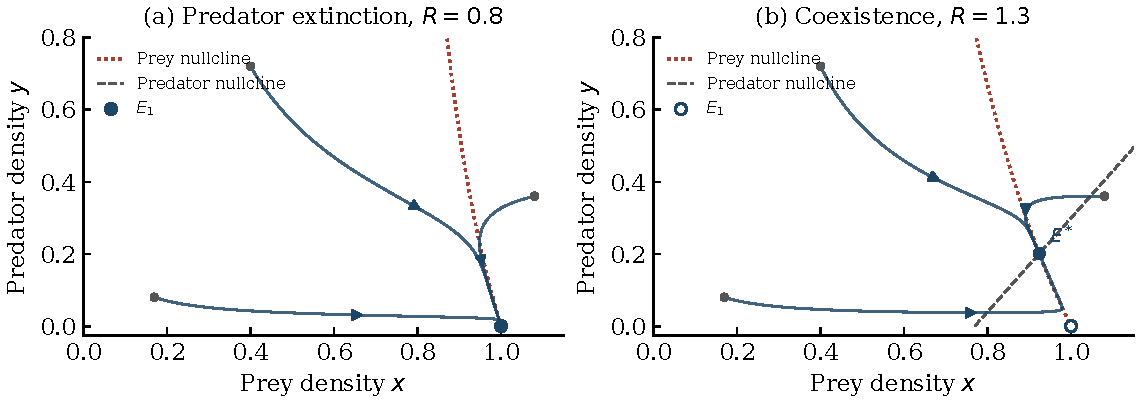
\includegraphics[width=\linewidth]{figures/num_invasion.pdf}
\caption{Phase portraits on the two sides of the invasion threshold, with the corresponding equilibrium and nullclines. Generated by \protect\path{code/numerical_study.py}.}
\label{fig:invasion}
\end{figure}

\subsection{Two stable coexistence states and a saddle boundary}
At \(m=3\) in the bistability case, the three feasible prey coordinates are approximately \(0.03542\), \(0.30000\) and \(0.56458\). The outer points attract, and the middle point is a saddle. In this case \(D=1.4\) exceeds \(M\chi(A)\simeq1.275\), so the basin theorem identifies the stable manifold as the common boundary. The starts \((0.12,14)\) and \((0.38,14)\) approach the low and high sinks, respectively. Figure~\ref{fig:basins} plots both trajectories and the boundary. The branch diagram varies \(m\) with the other inputs fixed, giving folds at \(m\simeq2.39552\) and \(m\simeq3.16069\).

\begin{figure}[!htbp]\centering
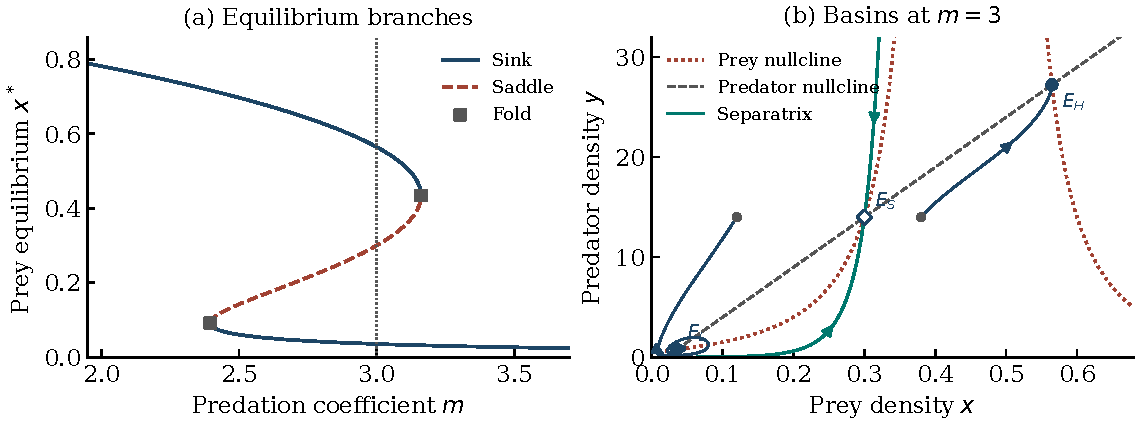
\includegraphics[width=\linewidth]{figures/num_basins.pdf}
\caption{Coexistence branches and phase portrait for the bistable case. The displayed separatrix is a numerical trace of the stable manifold of the middle saddle. Generated by \protect\path{code/numerical_study.py}.}
\label{fig:basins}
\end{figure}

\subsection{Predation and enrichment as Hopf parameters}
For the predation path the threshold is \(m_H=24/5\) at \((x^*,y^*)=(1/5,6/25)\). Its determinant is \(7/5\), its along-branch trace derivative is \(61/168\), and the cubic coefficient in the original-time convention is \(-1525/168\). For the enrichment path, \(k_H=1\) at \((x^*,y^*)=(1/10,162/1855)\). The corresponding values are \(49/25\), \(601/2520\) and \(-1415/252\). Both trace derivatives are positive and both cubic coefficients are negative. The crossings are supercritical. Figure~\ref{fig:hopf} shows phase portraits below and above each threshold. In the enrichment comparison only \(k\) varies, while \(\alpha\), \(m\), \(r\), \(\beta\), \(e\) and \(d\) remain fixed.

\begin{figure}[!htbp]\centering
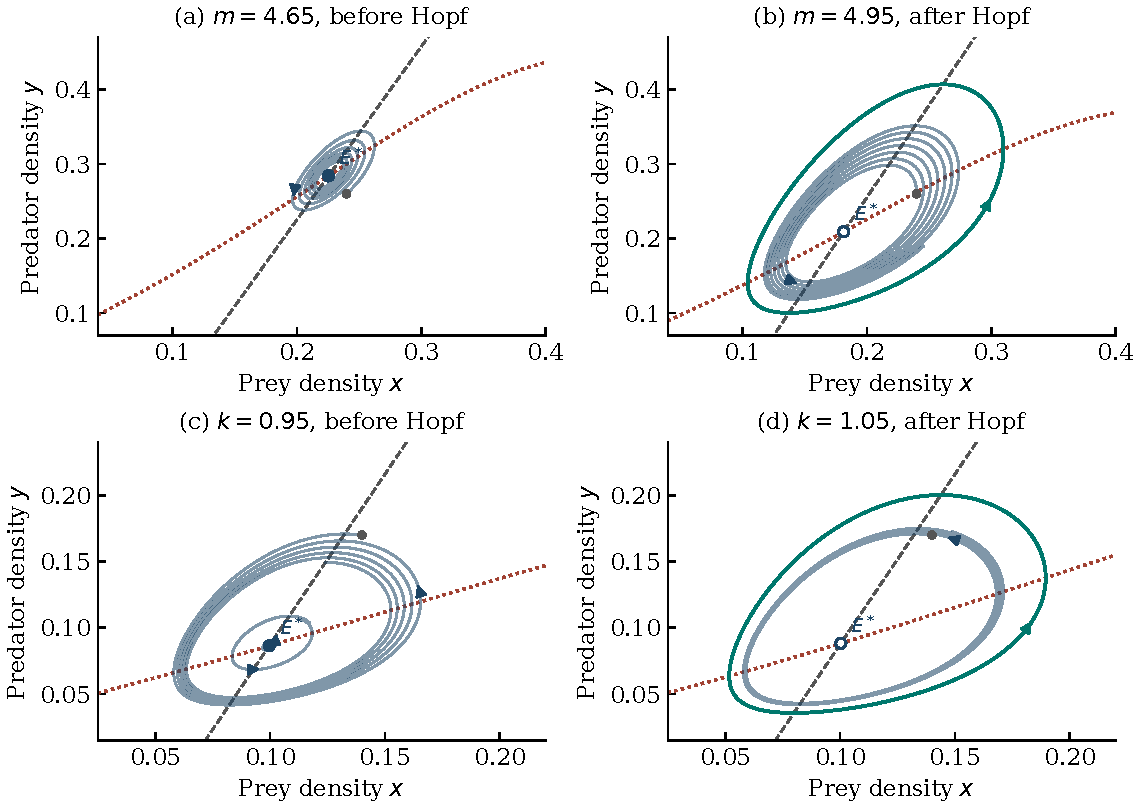
\includegraphics[width=\linewidth]{figures/num_hopf.pdf}
\caption{Phase portraits below and above the predation and enrichment Hopf thresholds. Thin lines show selected transient arcs. The green curve in the two cycling cases is the computed periodic orbit. Generated by \protect\path{code/numerical_study.py}.}
\label{fig:hopf}
\end{figure}

\subsection{Fold cusp and Bogdanov--Takens point}
The cusp in the \((m,\beta)\) plane is at \((3.7,4.5)\) for the inputs shown in Table~\ref{tab:constructed}. Its triple root is \(x^*=0.3\). Near it the fold curves separate regions with one and three feasible equilibria. For the Bogdanov--Takens example, \((m,k)=(17/5,1)\) and \((x^*,y^*)=(1/5,144/425)\). At the latter point \(Q=Q'=T=0\), the Jacobian has rank one, and the two quadratic normal-form coefficients are \(3\) and \(-13/12\). The unfolding determinant is \(-271/1224\). Figure~\ref{fig:two} displays the cusp folds and the local fold and trace-zero loci near the Bogdanov--Takens point. The trace-zero curve is shown where the determinant is positive. The regularity conditions also imply a local saddle-loop curve.

\begin{figure}[!htbp]\centering
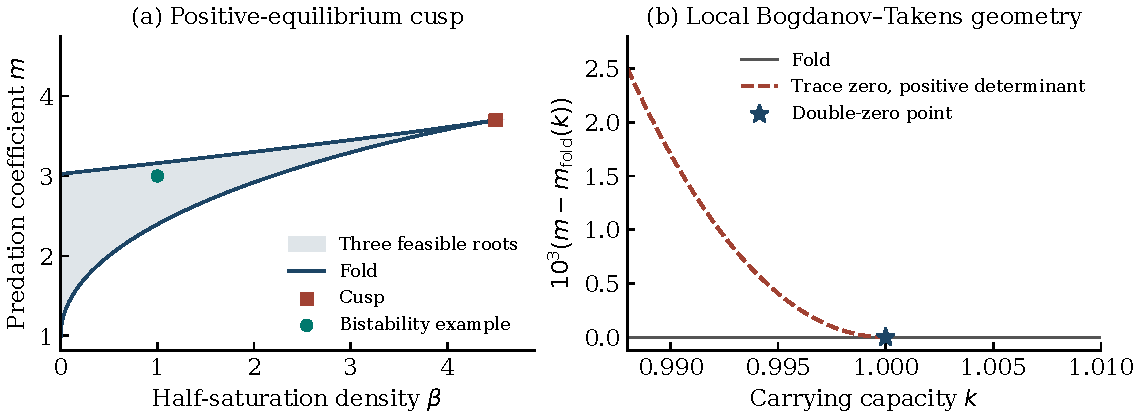
\includegraphics[width=\linewidth]{figures/num_two_parameters.pdf}
\caption{Two-parameter diagrams in the original model inputs. The cusp and the Bogdanov--Takens point arise on different parameter slices. Generated by \protect\path{code/numerical_study.py}.}
\label{fig:two}
\end{figure}

\subsection{A globally unique attracting orbit and a local cycle fold}
For the unique-cycle case \((A,M,R,D)=(10,12,5.5,3.5)\). The coexistence cubic strictly decreases on the strip, since \(p(X)+Xp'(X)\le3.7\) and \(M=12\). Its sole feasible root lies in \((0.21,0.27)\), where \(N>0\). Also \(M>\max p\). An exact Bernstein coefficient check of \(N'\mathcal Q-N\mathcal Q'\) on eight subintervals gives strict positivity on the full strip. The global uniqueness criterion therefore applies. Figure~\ref{fig:uniqueorbit} pairs the phase portrait with return diagnostics. The last section crossings from the three starts were within \(1.5\times10^{-7}\) of the computed crossing.

\begin{figure}[!htbp]\centering
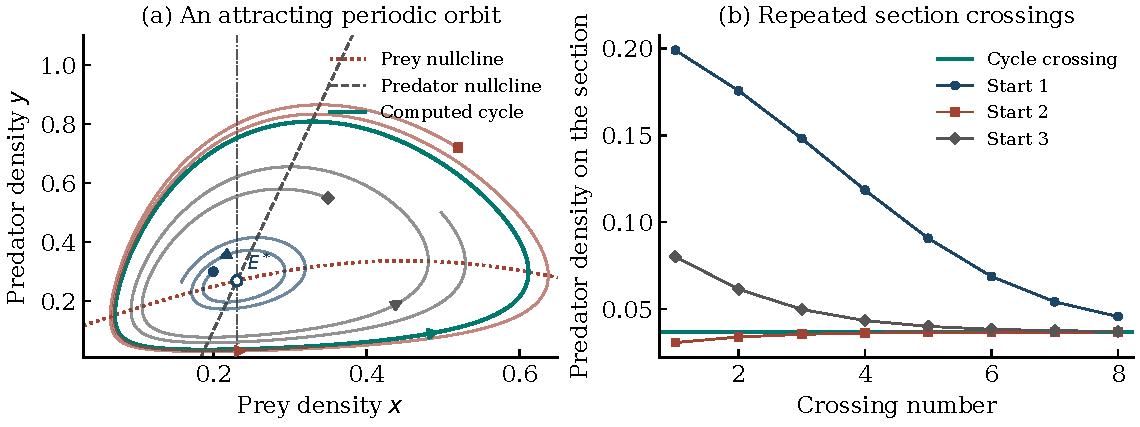
\includegraphics[width=\linewidth]{figures/num_cycle.pdf}
\caption{An attracting periodic orbit in the certified one-cycle region. A return-section calculation supplies the periodicity and attraction diagnostics. Generated by \protect\path{code/numerical_study.py}.}
\label{fig:uniqueorbit}
\end{figure}

Figure~\ref{fig:normalcycles} gives the separate local picture at supercritical Hopf and generalized Hopf. The generalized Hopf panel has two positive branches for \(-1/4<U<0\), one attracting and one repelling. The axes are scaled normal-form coordinates. Away from the organizing point, these curves do not give numerical amplitudes or a global count of periodic orbits for the population model.

\begin{figure}[!htbp]\centering
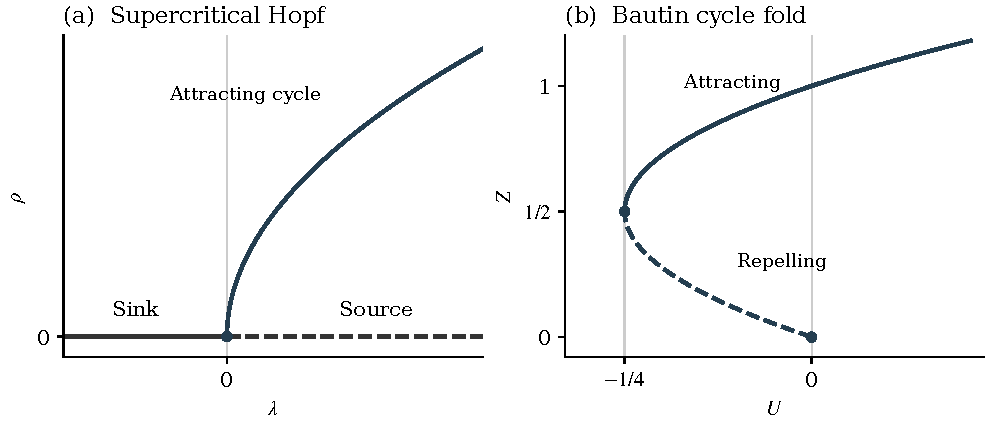
\includegraphics[width=\linewidth]{figures/analytical_cycles.pdf}
\caption{Local normal-form branches. At supercritical Hopf the stable cycle satisfies \(\rho^2=\lambda\). Near the generalized Hopf point the scaled cycle fold is \(U=Z^2-Z\). Solid branches are attracting and dashed branches repelling in the radial equation. Generated by \protect\path{code/analytical_diagram.py}.}
\label{fig:normalcycles}
\end{figure}

For a finite orbit calculation near the Bautin point, set \(r=k=\beta=1\), \(A=10\), \(s=0.1\), \(h_*=522/449+0.01\), and \(D=D_H+2\times10^{-5}\) in the Hopf family of Section~\ref{sec:family}. Then \(m\simeq3.335072\), \(e\simeq8.449066\) and \(d\simeq1.296992\). The low-density equilibrium is a stable focus. The directed return displacement on \(x=s\) changes sign in each of two disjoint brackets. Shooting gives an inner repelling orbit and an outer attracting orbit around this equilibrium. Figure~\ref{fig:bautin-numerical} shows the local configuration. A second stable focus and a saddle at higher prey densities lie outside the displayed region.

\begin{figure}[!htbp]\centering
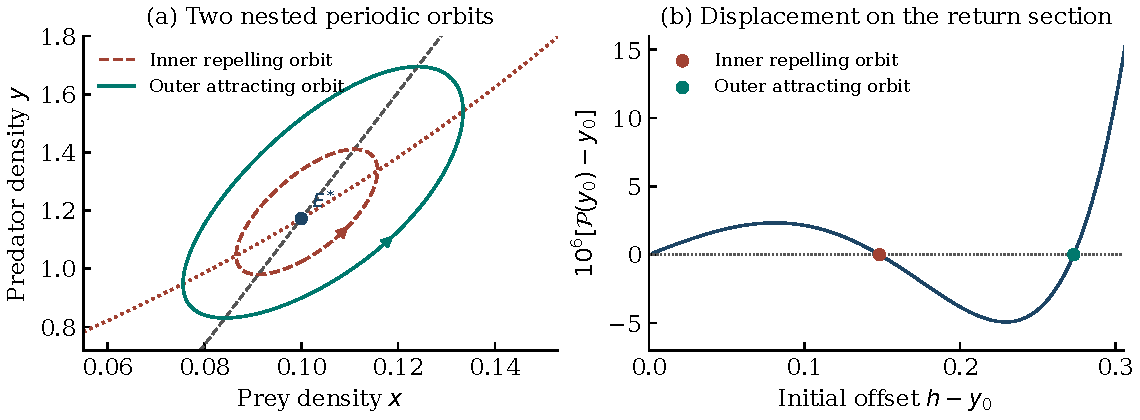
\includegraphics[width=\linewidth]{figures/num_bautin.pdf}
\caption{Two nested periodic orbits near generalized Hopf. The zeros of the return displacement correspond to the two curves in the phase plane. Here \(h\) in the axis label is the scaled predator equilibrium \(h_*\). Generated by \protect\path{code/numerical_study.py}.}
\label{fig:bautin-numerical}
\end{figure}

\begin{table}[!htbp]\centering
\caption{Periods and transverse multipliers at the computed periodic orbits. Every orbit closes to within \(1.3\times10^{-12}\) in the infinity norm after an independent Radau integration over its computed period.}
\label{tab:periods}
\begin{tabular}{@{}lrrl@{}}\toprule
Case & Period & Multiplier & Transverse stability\\ \midrule
Predation at \(m=4.95\) & 5.142344 & 0.79269272 & Attracting\\
Enrichment at \(k=1.05\) & 4.676835 & 0.94531264 & Attracting\\
Unique cycle & 2.882901 & 0.47852131 & Attracting\\
Bautin inner & 8.259431 & 1.00006672 & Repelling\\
Bautin outer & 8.381396 & 0.99973106 & Attracting\\
\bottomrule\end{tabular}
\end{table}

\subsection{Literature-informed prey growth rates}\label{sec:literature-cases}
Following \citet[Sec.~4, Table~6]{haque11}, we use the prey growth rates attributed to
\citet{tanner75}. Table~\ref{tab:lit-rates} separates the reported observed rates from
Tanner's estimates for optimal conditions. For all three species pairs we use
\(k=100,\ \alpha=0.04,\ m=1.20,\ \beta=10,\ e=0.25,\ d=0.30\), with time in years.
The choices of \(k\) and \(d\) match values used in Haque's numerical setup. The other
common inputs define a controlled comparison for Eq.~\eqref{eq:ode}. Tanner's predator
growth rates describe population increase and do not enter the mortality parameter \(d\).

\begin{table}[htbp]
\centering\small
\caption{Prey growth-rate intervals and results at the lower observed endpoint. Rate intervals
and the largest eigenvalue real part are in \(\mathrm{yr}^{-1}\). Tanner's maximum estimates
represent optimal conditions.}\label{tab:lit-rates}
\begin{tabular}{@{}lccccc@{}}
\toprule
Prey / predator & Observed & Maximum & \((x^*,y^*)\) & \(\max\Re\lambda\) & Type \\
\midrule
Muskrat / mink & 0.806--1.068 & 1.101--1.366 & (65.009, 55.009) & \(-0.30939\) & Node \\
Moose / wolf & 0.100--0.127 & 0.171--0.202 & (11.200, 1.200) & \(-0.00429\) & Focus \\
Snowshoe hare / lynx & 0.545--0.810 & 0.769--1.033 & (34.207, 24.207) & \(-0.08160\) & Focus \\
\bottomrule
\end{tabular}
\end{table}

The common inputs give \(R=10\), \(C=12\), \(C_{\rm crit}=6.25r\), and
\(d-m\chi(4)=0.06\). At the largest listed rate \(C_{\rm crit}=8.5375\), so the
unique-root and cycle-exclusion conditions guarantee global convergence throughout all
six intervals. The phase portraits in Fig.~\ref{fig:lit-rates} show a node for
muskrat/mink and damped oscillations for the other pairs at the lower observed rates.
The moose/wolf trajectory returns much more slowly at its lower rate. These comparisons
isolate the effect of \(r\) under the common inputs. The rate sweep includes both stable
nodes and stable foci in the observed hare interval. The remaining coefficients and initial
conditions are illustrative, so the trajectories give no estimates of wild population dynamics.

\begin{figure}[htbp]
\centering
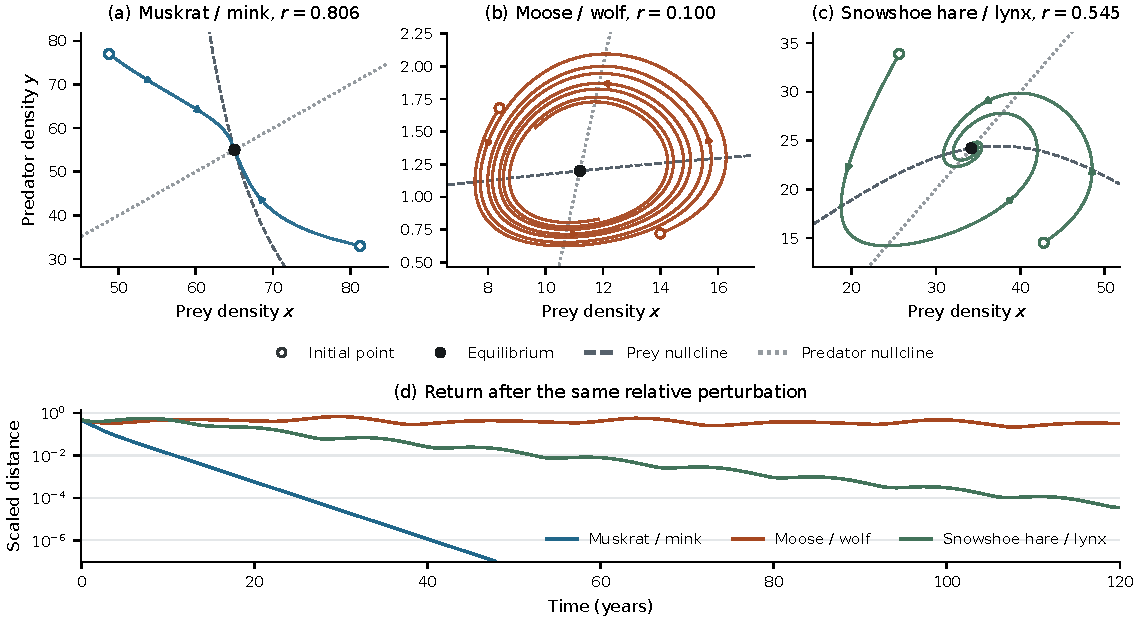
\includegraphics[width=\linewidth]{figures/lit_growth_rates.pdf}
\caption{Growth-rate comparison. Panels (a)--(c) use two initial points,
\((0.75x^*,1.4y^*)\) and \((1.25x^*,0.6y^*)\). Panel (d) shows the Euclidean distance in
\((x/x^*,y/y^*)\) from \((1,1)\) for the first initial point. The time span shown is
120 years. Python source \protect\texttt{code/literature\_cases.py}.}\label{fig:lit-rates}
\end{figure}

\FloatBarrier

\section{Stochastic stability near coexistence}\label{sec:noise}
Following Sections 3.3--3.4 of \citet{haque11}, we consider white and colored perturbations around a positive equilibrium. We work with local linear models and specify the noise separately from the deterministic system. Write \(u=((x-x^*)/k,(y-y^*)/\beta)^\top\), and let \(J\) be the Jacobian in these scaled density coordinates, with time \(t\) unchanged. Assume \(J\) is Hurwitz, meaning that both eigenvalues have negative real part.

\subsection{Independent multiplicative white noise}
Let \(W_1,W_2\) be independent standard Wiener processes. With coordinate projections \(P_i\) and noise intensities \(\sigma_i\), consider the It\^o system
\[
 \dd u=Ju\,\dd t+\sum_{i=1}^2 B_i u\,\dd W_i,\qquad B_i=\sigma_iP_i.
\]
Let \(P=P^\top>0\) solve \(J^\top P+PJ=-I\). It\^o's formula gives
\[
 \frac{\dd}{\dd t}\mathbb E[u^\top Pu]
 =-\mathbb E\!\left[u^\top
       \left(I-\textstyle\sum_i B_i^\top PB_i\right)u\right].
\]
Thus \(I-\sum_i B_i^\top PB_i>0\) is sufficient for exponential mean-square stability. If its smallest eigenvalue is \(\epsilon>0\), the right side is at most \(-\epsilon\,\mathbb E[u^\top Pu]/\lambda_{\max}(P)\). The eigenvalue bounds on \(P\) then give exponential decay of \(\mathbb E\|u(t)\|^2\). The plotted moments are obtained from the exact matrix equation \(\dot C_u=JC_u+C_uJ^\top+\sum_iB_iC_uB_i^\top\), where \(C_u=\mathbb E[uu^\top]\).

\subsection{A common Ornstein--Uhlenbeck fluctuation}
To obtain an explicit colored-noise bound, let a common scalar fluctuation \(\xi(t)\) modulate both coordinates, so \(\dot u=(J+\xi I)u\). Take \(\xi\) to be a stationary, mean-zero Ornstein--Uhlenbeck process with variance \(q>0\) and covariance \(q e^{-\theta |t-s|}\), \(\theta>0\). For fixed \(u(0)\), the matrices commute and hence
\[
 u(t)=e^{Jt}u(0)\exp\!\left(\int_0^t \xi(s)\,\dd s\right),\qquad
 V_\xi(t)=2q\left[\frac{t}{\theta}-\frac{1-e^{-\theta t}}{\theta^2}\right],
\]
where \(V_\xi(t)\) is the variance of the integral. The Gaussian exponential moment gives \(\mathbb E\|u(t)\|^2=e^{2V_\xi(t)}\|e^{Jt}u(0)\|^2\). If \(2q/\theta<-\max\Real\operatorname{spec} J\), choose \(\gamma\) strictly between these values. Since \(\|e^{Jt}\|\le K_\gamma e^{-\gamma t}\), the second moment decays exponentially. This condition applies to the stated common modulation of the local linear system.

\subsection{A numerical check}
At \((r,k,\alpha,m,\beta,e,d)=(1,10,0.2,1.76,1,1/6,0.88)\), the coexistence equilibrium is \((6,1)\) and the largest real part of the Jacobian eigenvalues is \(-0.64\). For \((\sigma_1,\sigma_2)=(0.35,0.45)\), the minimum eigenvalue in the white-noise dissipation test is \(0.803895\). For \((q,\theta)=(0.12,1.2)\), the colored-noise threshold gives \(2q/\theta=0.2<0.64\). The white-noise moment calculation agrees with a separate integration of the moment equation to \(5.8\times10^{-15}\) in absolute error. Numerical quadrature of the colored-noise covariance agrees with the closed variance at the five checked times to \(2.3\times10^{-16}\).

\begin{figure}[!htbp]\centering
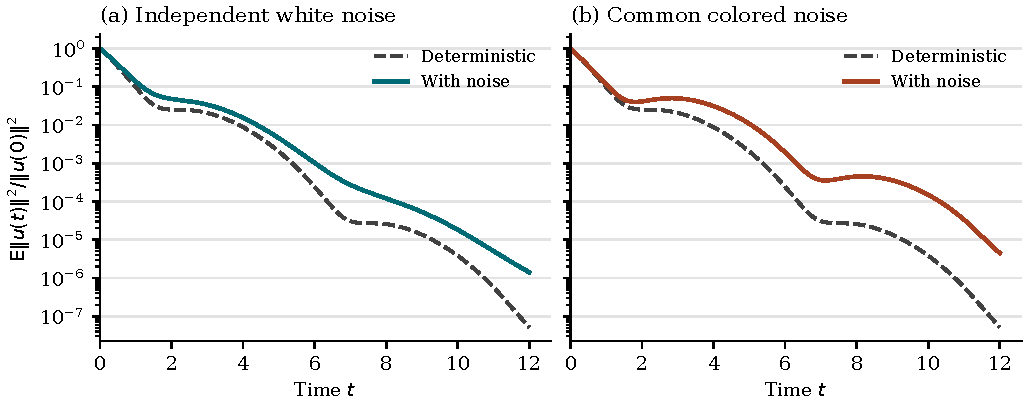
\includegraphics[width=\linewidth]{figures/stoch_moments.pdf}
\caption{Second moments for the two local perturbation models, both starting at \(u(0)=(0.01,-0.02)^\top\). A logarithmic axis shows the decay compared with the deterministic displacement. The curves come from the moment equations and the integrated Gaussian variance. Generated by \protect\path{code/stochastic_stability.py}.}\label{fig:noise}
\end{figure}

\section{Discussion and conclusions}\label{sec:discussion}
The invasion threshold separates the conditions for coexistence from the kind of coexistence that follows. For \(R\le1\), every positive trajectory approaches the predator-free state. At equality the decay of the predator is of order \(t^{-1}\). For \(R>1\), both species persist. The analysis of \(F(x)+C/x\) explains how an increase in prey growth at low density can lead to three feasible equilibria. When the outer equilibria attract and cycles are excluded, the initial populations determine the long-run state through their position relative to the saddle separatrix.

The parameters \(\alpha\) and \(\beta\) influence distinct parts of this mechanism. Increasing \(\alpha\) increases the initial slope of per-capita prey growth and can permit the turning points of the equilibrium curve. Increasing \(\beta\), with other dimensional inputs fixed, lowers the predator invasion ratio and changes the constant term of the coexistence cubic. These statements concern the current response \(mxy/(\beta+y)\), whose interpretation follows directly from that denominator. The displayed predator equation has no separate quadratic mortality term. Adding such a term changes the predator nullcline and requires recalculating both the root and stability conditions.

The Hopf cases show that varying either predation or carrying capacity can destabilize a coexistence equilibrium and produce local attracting oscillations along specified parameter paths. For enrichment this agrees qualitatively with one mechanism discussed by \citet{haque11}; the transition depends on the parameter path and the response function. The numerical loss of stability does not itself predict predator extinction or establish the large-amplitude fate of a periodic branch. Conversely, a periodic trajectory obtained by integration does not prove uniqueness. Our one-orbit case uses a separate global criterion with its hypotheses checked at the chosen inputs.

The literature-informed results show how changing \(r\) affects equilibrium levels and transient shapes under a common illustrative setting. A field prediction would require independent estimates of predation, conversion, interference, mortality and observation scales for each species pair. The stochastic results concern small displacements about a coexistence state in the two stated noise models. The global count of cycles outside the certified regions, continuation far from the codimension-two points, and the zero-trace triple root remain open here.

\clearpage
\appendix
\section{Formula sheet and figure code}\label{sec:figurecode}
\begin{table}[!htbp]\centering
\caption{Quantities used to move from a parameter set to the corresponding stability test.}
\label{tab:formulasheet}
\begin{tabularx}{\linewidth}{@{}lY@{}}\toprule
Quantity & Definition and use\\ \midrule
Invasion & \(R=emk/(d\beta)\). The predator grows when rare at \(E_1\) precisely when \(R>1\).\\
Coexistence & \(Q(x)=x[F(x)-m]+C\) with \(C=d\beta/e\). Keep roots \(C/m<x<k\) and set \(y=emx/d-\beta\).\\
Local stability & \(T=xF'(x)-dF(x)/m\) and \(\Det=-(dF(x)/m)Q'(x)\) at a feasible root.\\
Cycle exclusion & \(A=\alpha k\), \(M=m/r\), \(D=d/r\). The first Dulac bound is \(D\ge M\chi(A)\).\\
Hopf threshold & At a simple equilibrium, \(T=0\) and \(\Det>0\). Check the along-branch crossing derivative and the cubic focal coefficient.\\
\bottomrule\end{tabularx}
\end{table}

The paths in Table~\ref{tab:figurepaths} are relative to the root of the accompanying source package. Its data directory contains machine-readable parameter sets and numerical diagnostics. The figure scripts regenerate the plots from the model and the recorded inputs.

\begin{table}[H]\centering
\caption{Python entry points for all figures in this report.}
\label{tab:figurepaths}
\begin{tabularx}{\linewidth}{@{}cYY@{}}\toprule
Figure & Output under \texttt{figures/} & Python entry point\\ \midrule
\ref{fig:invasion} & \path{num_invasion.pdf} & \path{code/numerical_study.py}\\
\ref{fig:basins} & \path{num_basins.pdf} & \path{code/numerical_study.py}\\
\ref{fig:hopf} & \path{num_hopf.pdf} & \path{code/numerical_study.py}\\
\ref{fig:two} & \path{num_two_parameters.pdf} & \path{code/numerical_study.py}\\
\ref{fig:uniqueorbit} & \path{num_cycle.pdf} & \path{code/numerical_study.py}\\
\ref{fig:normalcycles} & \path{analytical_cycles.pdf} & \path{code/analytical_diagram.py}\\
\ref{fig:bautin-numerical} & \path{num_bautin.pdf} & \path{code/numerical_study.py}\\
\ref{fig:lit-rates} & \path{lit_growth_rates.pdf} & \path{code/literature_cases.py}\\
\ref{fig:noise} & \path{stoch_moments.pdf} & \path{code/stochastic_stability.py}\\
\bottomrule\end{tabularx}
\end{table}

\clearpage
\bibliographystyle{elsarticle-harv}
\bibliography{references}
\clearpage
\section{Research Extensions}\label{sec:extensions}
\noindent\textbf{1. How does the feeding law change coexistence?}\par
We kept the coursework's weak Allee prey growth and changed only the feeding law. All five models preserve positive populations and keep them bounded. In the two prey-dependent models (P1 and P2), positive coexistence fixes prey density independently of carrying capacity. The original foraging-arena response (P0) can support two attracting coexistence states. With ratio-dependent feeding (P4), enrichment lowers the Jacobian trace at every positive coexistence state with positive determinant for the coursework growth law. For a positive growth factor $g$ with $g'>0$, the same decrease holds at a given prey density for every admissible ratio-dependent intake if and only if $(1/g)''\geq0$ there.

\medskip
\noindent\textbf{2. How do prey growth and predator competition interact?}\par
We kept the feeding law fixed and paired three prey growth laws with and without direct predator competition. Logistic growth allows at most one positive equilibrium. Weak and strong Allee growth can each support three. When the three growth laws are calibrated to the same coexistence state at zero competition, positive competition orders predator density along their common branches with positive determinant. Predator density is highest for strong Allee growth, intermediate for weak Allee growth, and lowest for logistic growth. This ranks equilibrium levels even when predator density falls in all three models. In 48 disturbance simulations at the study baseline, 45 recovered. All three failures followed prey removal under strong Allee growth.

\medskip
\noindent\textbf{3. What transfers when the same equation is fitted to other systems?}\par
We kept the ecological equation and fitted its coefficients to training conditions in tumor--T-cell and bacteria--phage datasets. The equation had lower mean held-out error than the CARRGO model on the PBT138 cell line, while the infection-stage model had lower four-hour error in 11 of 12 $\lambda$-phage conditions. In 12 held leukemia conditions, fitting targets alone predicted none of the observed early T-cell increases. Fitting both populations predicted all 12, but mean target root-mean-square error rose from 81,634 to 197,580 cells. The measured trade-off concerns predictions for held conditions from this dataset.

\medskip

\noindent The companion \textit{Appendix --- Research Extensions} gives the figures, proofs, Python calculations, and Lean verification results for each study.
\end{document}

